Når data fra databasen skal tilgås, benyttes Repository-pattern og UnitOfWork, der er beskrevet i afsnit \ref{Manglende reference}. 
Det betyder, at når data skal hentes i databasen skal der først oprettes et GenericRepository af den benyttede type. Dette genericRepository benyttes som et håndtag til databasen, når der skal hentes data.
Et sekvensdiagram, for hvordan for eksempel en barterad findes i databasen ved brug af både UnitOfWork og GenericRepository, kan ses på figur \ref{fig:UOFFindBarterAd}

\begin{figure}[H]
	\centering
	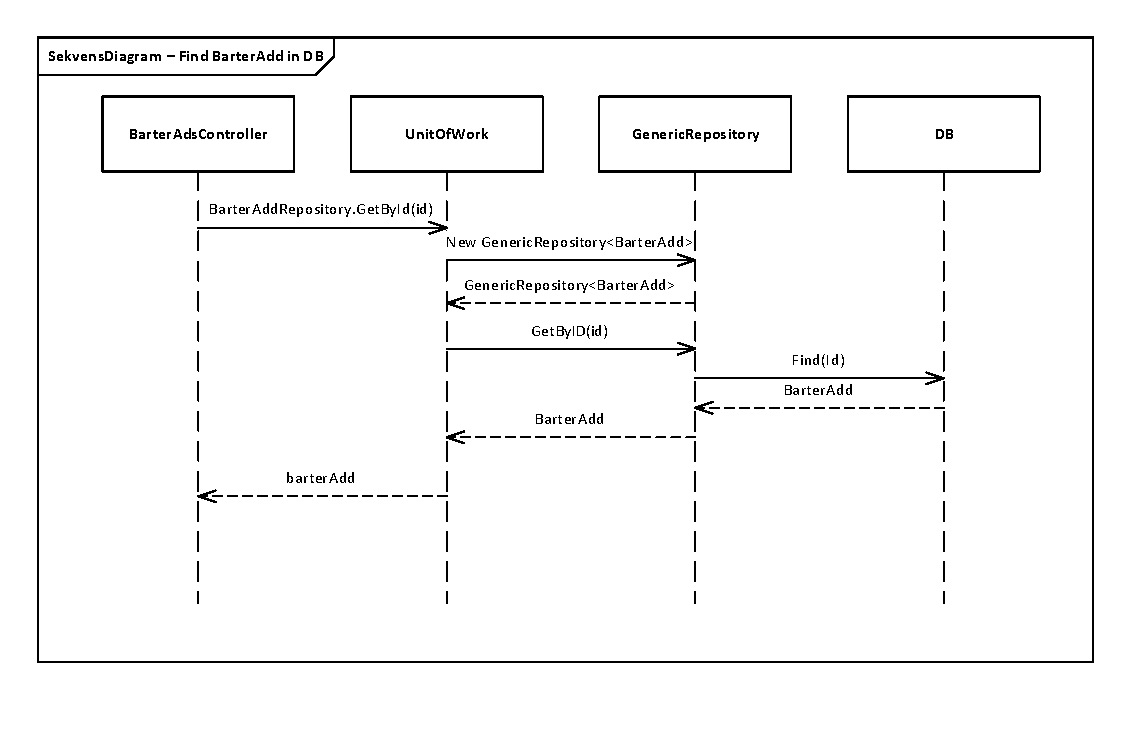
\includegraphics
	[width=140mm]{figures/SDUOFFindBarterAd.PDF}
	\caption{Sekvensdiagram for, hvordan en barterAd bliver fundet i DB}
	\label{fig:UOFFindBarterAd}
\end{figure}
På sekvensdiagrammet figur \ref{fig:UOFFindBarterAd} ses det, hvordan controlleren kalder over i unitofwork, der opretter et nyt genericrepository. Dette genericrepository finder barteraden i databasen.  



\begin{figure}[H]
	\centering
	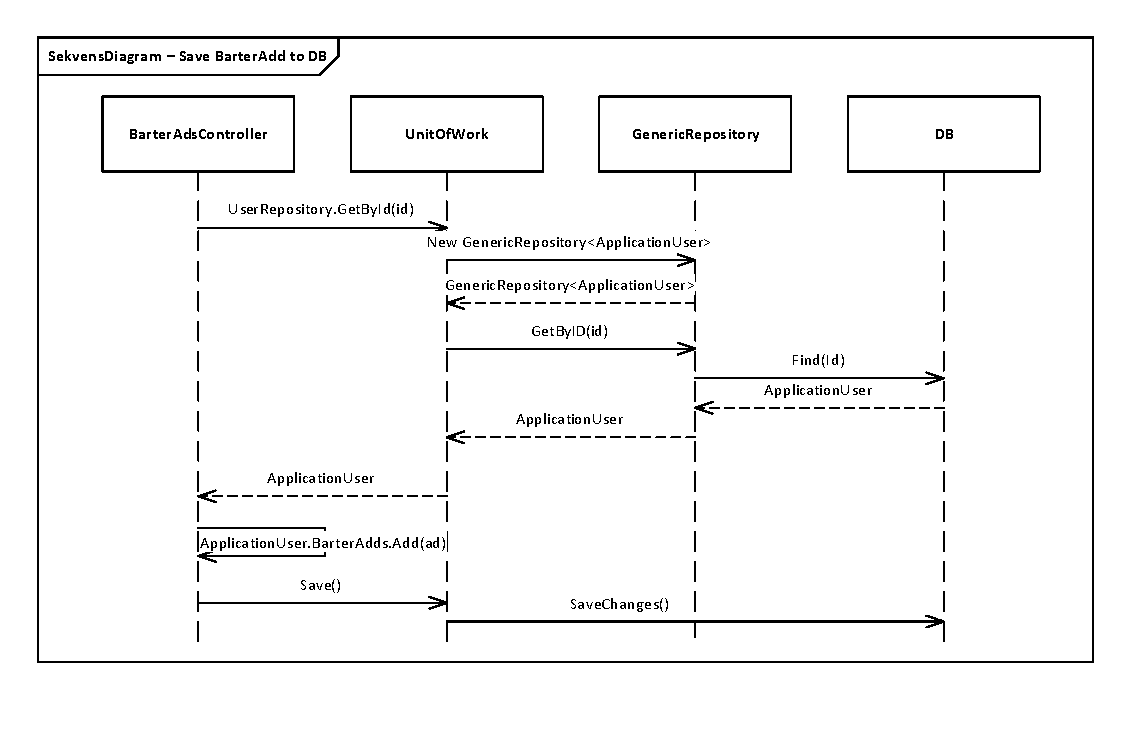
\includegraphics
	[width=140mm]{figures/SDUOFSaveBarterAd.PDF}
	\caption{Sekvensdiagram for, hvordan en barterAd bliver oprettet og gemt i DB}
	\label{fig:UOFSaveBarterAd}
\end{figure}